\documentclass[a4paper,12pt]{book}
\usepackage[utf8]{inputenc}
\usepackage{graphicx}
\usepackage{titlesec}
\usepackage{hyperref}

\titleformat
{\chapter} % command
[display] % shape
{\bfseries\Huge\itshape} % format
{\small{Tic-Tac-Toe Machine Learning Workshop}} % label
{0.5ex} % sep
{
	\rule{\textwidth}{1pt}
	\vspace{1ex}
	\centering
} % before-code
[
\vspace{-0.5ex}%
\rule{\textwidth}{0.3pt}
] % after-code





% Default fixed font does not support bold face
\DeclareFixedFont{\ttb}{T1}{txtt}{bx}{n}{12} % for bold
\DeclareFixedFont{\ttm}{T1}{txtt}{m}{n}{12}  % for normal

% Custom colors
\usepackage{color}
\definecolor{deepblue}{rgb}{0,0,0.5}
\definecolor{deepred}{rgb}{0.6,0,0}
\definecolor{deepgreen}{rgb}{0,0.5,0}

\usepackage{listings}

% Python style for highlighting
\newcommand\pythonstyle{\lstset{
		language=Python,
		basicstyle=\ttm,
		otherkeywords={self},             % Add keywords here
		keywordstyle=\ttb\color{deepblue},
		emph={MyClass,__init__},          % Custom highlighting
		emphstyle=\ttb\color{deepred},    % Custom highlighting style
		stringstyle=\color{deepgreen},
		frame=tb,                         % Any extra options here
		showstringspaces=false            % 
}}


% Python environment
\lstnewenvironment{python}[1][]
{
	\pythonstyle
	\lstset{#1}
}
{}

% Python for external files
\newcommand\pythonexternal[2][]{{
		\pythonstyle
		\lstinputlisting[#1]{#2}}}

% Python for inline
\newcommand\pythoninline[1]{{\pythonstyle\lstinline!#1!}}

\begin{document}
	
	\author{Martin Mrugała\\Patryk Walczak\\Filip Szymczak\\Bartek Żyła\\Maciej Zalewski}
	\title{\Huge{\bf{Machine Learning Workshop\\Tic-Tac-Toe Project}}}
	\date{\emph{\today}}
	
	\frontmatter
	\maketitle

	\tableofcontents
	
	\mainmatter
	\chapter{Introduction}
	\section{Standard Tic-tac-toe}
	According to the definition in the Oxford Dictionary of English, Tic-tac-toe is a game in which two players seek to complete a row of either three noughts or three crosses drawn alternately in the spaces of a grid of nine squares.
		\begin{figure}[!h]
		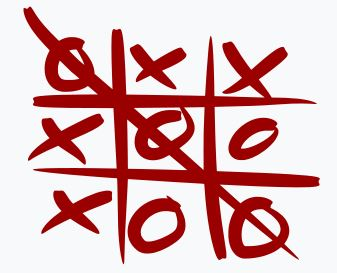
\includegraphics{./Images/1.jpg}
		\centering
		\caption{A completed game of Tic-tac-toe\protect\footnotemark.}
		\label{fig:Capture1}
	\end{figure}
	\footnotetext{Source of the image: \url{https://en.wikipedia.org/wiki/Tic-tac-toe}}
	And as it turns out, there are 255 168 possible games. So this means that, with the help of the reinforcement learning, a bot may train to mastery. 
	\newpage
	\section{Our implementation}
	Our team decided to create a bot which would play this game but in an expanded version of it. The principal changes concern, inter alia:\\
	\begin{itemize}
		\item \textbf{The size of the grid could be infinite}\\
		The number of squares is not boundless, of course. Due to the CPU, as well as the storage limitations, the infinity has to be simulated. We came up with two solutions. The first one is pretty straightforward, but a little preachy. The idea is to set the size in advance. The second one, in turn, assumes an increase in the size whenever the players get close to the edge.
		\item \textbf{Condition of winning}\\
		The length of the sequence of X's or O's needed to win may have any value. Naturally, it has to satisfy the following condition:
		\begin{center}
			$0 < length < edgelength$
		\end{center}
		There is still the matter of the draw. In case of the constant size gird, the tie occurs, whenever there is no way for any player to win.
	\end{itemize}
	\section{Machine Learning backgroud}
	\chapter{Code}
	\begin{python}
		class MyClass(Yourclass):
		def __init__(self, my, yours):
		bla = '5 1 2 3 4'
		print bla
	\end{python}
	\chapter{Bibliography}

	
	\backmatter
	% bibliography, glossary and index would go here.
	
\end{document}